\documentclass[mp2i]{exam}
\usepackage{draw}
\usepackage{base}
\usepackage{code}

\td{Graphe : Représentations et parcours}

\begin{document}
	\section{Représentations}
	\begin{enumerate}
		\item Écrire des fonctions \ocaml{mat_of_list : int list array -> int array array} et \\
		\ocaml{list_of_mat : int array array -> int list array} pour passer de liste d'adjacence à matrice d'adjacence et inversement. Quelles sont leurs complexités?
		\if\cor1
		\\$\blacktriangleright$~ Les fonctions suivantes sont quadratiques en le nombre de sommets:
		\begin{center}
			\fbox{\includegraphics[scale=.21]{img/mat_of_list.png}}\hspace{.1cm}
			\fbox{\includegraphics[scale=.21]{img/list_of_mat.png}}
		\end{center}
		\fi 
		\item Soit $\vec{G} = (V, \vec{E})$ un graphe orienté représenté par une matrice d'adjacence \ocaml{m : int array array}. \\
		Écrire une fonction \ocaml{trou_noir m} renvoyant en {O($\vert V \vert$)} un sommet $t$ vérifiant:
		\begin{itemize}
			\item[$\bullet$] $(u, t) \in \vec{E}$, $\forall u \neq t$
			\item[$\bullet$] $(t, v) \notin \vec{E}$, $\forall v \neq t$
		\end{itemize}  
		On supposera dans un premier temps que ce sommet existe, puis on expliquera comment le déterminer. 
		\if\cor1
		\\$\blacktriangleright$~ On conserve un candidat $c$ pour être trou noir (initialement 0) que l'on compare au sommet suivant $v$: s'il y a un arc ($c$, $v$) alors $v$ devient le candidat.
		\begin{center}
			\fbox{\includegraphics[scale=.21]{img/trou_noir.png}}
		\end{center}
		\ocaml{trou_noir g 0 1} renvoie le seul sommet qui peut être un trou noir. On peut ensuite vérifier que c'est bien un trou noir en O($\vert V \vert$).
		\fi 
		\item Écrire une fonction \ocaml{arb_of_pere : int array -> int arb} qui transforme en temps linéaire un arbre représenté par un tableau des pères (par exemple l'arbre de parcours en largeur/profondeur) en un arbre persistant (\ocaml{type 'a arb = N of 'a * 'a arb list}). La racine est son propre père.
		\if\cor1
		\\$\blacktriangleright$~ On peut construire un tableau des fils: \ocaml{fils.(i)} va être la liste des fils du sommet \ocaml{i}. Il est ensuite facile d'en déduire l'arbre correspondant. On utilise \ocaml{map f [u0; u1; ...]} qui renvoie \ocaml{[f u0; f u1; ...]}:
		\begin{center}
			\fbox{\includegraphics[scale=.21]{img/arb_of_pere.png}}
		\end{center}
		\fi 
		\item Quel est le nombre de chemins de longueur 100 de 0 à 2 dans le graphe orienté suivant?
		\begin{center}
			\tikz[>=latex] \graph [simple necklace layout,nodes={circle, draw}, node distance = 2cm] {
				0 ->[right] 1;
				1 -> 2;
				0 ->[loop left] 0;
				1 ->[loop left] 1;
				2 ->[loop right] 2;
			};
		\end{center}
		\if\cor1
		$\blacktriangleright$~ Sa matrice d'adjacence est $A = \begin{pmatrix}
		1 & 1 & 0\\
		0 & 1 & 1 \\
		0 & 0 & 1
		\end{pmatrix}$. Alors $A^n = (\underbrace{\begin{pmatrix}
		1 & 0 & 0\\
		0 & 1 & 0 \\
		0 & 0 & 1
		\end{pmatrix}}_I + \underbrace{\begin{pmatrix}
		0 & 1 & 0\\
		0 & 0 & 1 \\
		0 & 0 & 0
		\end{pmatrix}}_J)^n = I + n J + \binom{n}{2}J^2$. \\
	Le nombre demandé est donc $\binom{100}{2}$.  
		\fi 
		\item Comment déterminer si un graphe possède un cycle de longueur $k$ en utilisant sa matrice d'adjacence $A$? On en déduit par exemple un algorithme pour déterminer si un graphe est sans triangle (cf TD 1).
		\if\cor1
		\\$\blacktriangleright$~ Un coefficient diagonal $(a_{i, i}^{(k)})$ de $A^k$ correspond au nombre de cycles de longueur $k$ passant par le sommet $i$.  
		\fi 
		\item Comment déterminer le nombre de chemins \textbf{élémentaires} (qui ne reviennent pas sur le même sommet) de longueur $k$ en utilisant la matrice d'adjacence? 
		\if\cor1
		\\$\blacktriangleright$~ Il suffit de mettre à 0 la diagonale à chaque calcul de puissance.
		\fi 
		\item Soit $G$ un graphe non-orienté \textbf{$\boldsymbol{k}$-régulier} (dont tous les sommets ont degré $k$). Montrer que $k$ est valeur propre de la matrice d'adjacence $A$ de $G$. Quelle propriété similaire a-t-on pour les graphes orientés?
		\if\cor1
		\\$\blacktriangleright$~ si $v_1$, ..., $v_n$ sont les sommets correspondants aux lignes de $A$, $A \begin{pmatrix}
		1 \\
		\vdots \\
		1
		\end{pmatrix} = \begin{pmatrix}
		\deg(v_1) \\
		\vdots \\
		\deg(v_n)
		\end{pmatrix} = k \begin{pmatrix}
		1 \\
		\vdots \\
		1
		\end{pmatrix}$.
		\fi 
		\item Quelles sont les valeurs propres possibles de la matrice d'adjacence $A$ d'un graphe orienté sans cycle?
		\if\cor1
		\\$\blacktriangleright$~ Si $n$ est le nombre de sommets, la longueur d'un chemin est au plus $n - 1$ (sinon il y aurait un cycle). Donc $A^n = 0$: $X^n$ est annulateur de $A$ donc la seule valeur propre possible de $A$ est 0.
		\fi 
	\end{enumerate}
		
	\section{Distances}
	Soit $G = (V, E)$ un graphe. On rappelle que la \textbf{distance} de $u$ à $v$ est la longueur minimum d'un chemin de $u$ à $v$ (c'est aussi une distance au sens mathématiques, pour un graphe non-orienté).
	\begin{enumerate}
		\item L'\textbf{excentricité} d'un sommet $u$ est la distance maximum de ce sommet à un autre. Écrire une fonction \\ \ocaml{exc : int graph -> int -> int} renvoyant en O($\vert V \vert + \vert E \vert$) l'excentricité d'un sommet.
		\if\cor1
		\\$\blacktriangleright$~ On renvoie la distance du dernier sommet visité par un BFS:
		\begin{center}
			\fbox{\includegraphics[scale=.21]{img/exc.png}}
		\end{center}
		\fi 
		\item Écrire une fonction \ocaml{diametre : int graph -> int} renvoyant en O($\vert V \vert \times (\vert V \vert + \vert E \vert)$) le \textbf{diamètre} d'un graphe, c'est à dire la distance maximum entre deux sommets.
		\if\cor1
		\\$\blacktriangleright$~ On cherche l'excentricité maximum. \ocaml{diametre 0} est la fonction demandée:
		\begin{center}
			\fbox{\includegraphics[scale=.21]{img/diametre.png}}
		\end{center}
		\fi 
		\item Écrire une fonction \ocaml{centre : int graph -> int} renvoyant en O($\vert V \vert \times (\vert V \vert + \vert E \vert)$) le \textbf{centre} d'un graphe, c'est à dire le sommet d'excentricité minimum.
		\if\cor1
		\\$\blacktriangleright$~ On peut renvoyer à la fois l'excentricité min et le sommet correspondant:
		\begin{center}
			\fbox{\includegraphics[scale=.21]{img/centre.png}}
		\end{center}
		\fi 
		\item Peut-on améliorer les trois algorithmes précédents si $G$ est un arbre?
		\if\cor1
		\\$\blacktriangleright$~ On peut trouver le diamètre d'un arbre en O($\vert V \vert$ + $\vert E \vert$): \\
		\underline{1ère solution}: convertir $G$ en \ocaml{int arb} (avec \ocaml{arb_of_pere} du I appliqué sur le tableau des pères d'un parcours de $G$) puis utiliser le fait que le diamètre de \ocaml{N(r, a::q)} est soit le diamètre de \ocaml{a}, soit le diamètre de \ocaml{N(r, q)}, soit la hauteur de \ocaml{a} + la hauteur de \ocaml{N(r, q)}. Puisqu'on a besoin du diamètre et de la hauteur, on renvoie un couple (diamètre, hauteur):
		\begin{center}
			\fbox{\includegraphics[scale=.21]{img/diam_tree.png}}
		\end{center}
		\underline{2ème solution}: faire un BFS depuis un sommet quelconque (ici 0), puis refaire un BFS depuis le dernier sommet visité. On peut montrer que la dernière distance obtenue est le diamètre (ceci ne marche qu'avec un arbre).
		\begin{center}
			\fbox{\includegraphics[scale=.21]{img/bfs1.png}}
		\end{center}
		On peut montrer que le milieu d'un chemin réalisant le diamètre d'un arbre est un centre (exercice). On pourrait donc calculer le centre d'un arbre en temps linéaire. 
		\fi 
		\item Soient $S \subset V$ et $T \subset V$. Comment calculer efficacement la distance entre $S$ et $T$, c'est à dire la distance minimum entre un sommet de $S$ et un de $T$?
		\if\cor1
		\\$\blacktriangleright$~ \underline{1ère solution}: rajouter deux sommets $s$ et $t$ reliés à tous les sommets de $S$ et $T$ respectivement. La distance entre $S$ et $T$ est alors celle entre $s$ et $t$ moins 2.\\
		\underline{2ème solution}: faire un BFS en initialisant la couche \ocaml{cur} en cours avec tous les sommets de $S$. On s'arête dès qu'on trouve un sommet de $T$. 
		\fi 
		\item Soient $u, v, w \in V$. Comment trouver efficacement un plus court chemin de $u$ à $w$ passant par $v$?
		\if\cor1
		\\$\blacktriangleright$~ On peut faire un BFS depuis $v$ pour en déduire un plus court chemin de $u$ à $v$ et un plus court chemin de $v$ à $w$, qu'on concatène.
		\fi 
		\item Soit $G = (V, E)$ et $k \in \mathbb{N}$ tel que $\deg(v) \leq k$, $\forall v \in V$. Soient $u, v \in V$. Expliquer comment trouver la distance $d$ de $u$ à $v$ en O($\sqrt{k^{d}}$). Comment procéder pour un graphe orienté?
		\if\cor1
		\\$\blacktriangleright$~ Un BFS va visiter au plus 1 + $k$ + $k^2$ + ... + $k^p$ = $\frac{k^{p+1} - 1}{k - 1}$ = O($k^p$) sommets à profondeur $p$. On peut faire partir simultanément deux BFS: un depuis $u$ et l'autre depuis $v$. Au moment où ils se << rejoignent >>, la somme des profondeurs des BFS est égale à la distance de $u$ à $v$. Le nombre total de sommets visités est au plus O($k^{\frac{d}{2}}$) + O($k^{\frac{d}{2}}$) = O($k^{\frac{d}{2}}$).
		\fi 
		%\item Expliquer comment trouver le plus court cycle d'un graphe en O($\vert V \vert$ $\times$ ($\vert V \vert + \vert E \vert$)).
	\end{enumerate}
	\if\cor0 \newpage \fi
	
	\section{Composantes fortement connexes}
	Dans tout l'exercice, \ocaml{g : int list array} est un graphe orienté représenté par liste d'adjacence.
	\subsection{Tri topologique}
	\begin{enumerate}
		\item Écrire une fonction \ocaml{post_dfs g vu r} renvoyant la liste des sommets atteignables depuis \ocaml{r} dans l'ordre de fin de traitement croissant d'un DFS (c'est à dire dans l'ordre postfixe/suffixe de l'arbre de parcours en profondeur). \ocaml{vu} est un tableau des sommets déjà visités. On pourra utiliser \ocaml{@} pour simplifier l'écriture.
		\if\cor1
%		\\$\blacktriangleright$
		\code{img/post_dfs.png}
		\fi 
		\begin{figure}[h!]
			\centering
			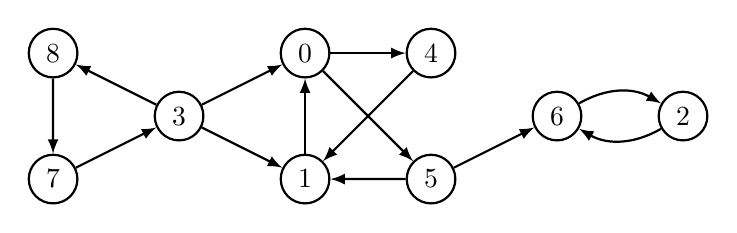
\begin{tikzpicture}[every node/.style={draw,thick,circle}, scale=.8, every path/.style={thick, ->, >=latex}]
			\node (3) at (-2, -1) {3};
			\node (7) at (-4, -2) {7};
			\node (8) at (-4, 0) {8};
			\node (0) at (0, 0) {0};	
			\node (4) at (2, 0) {4};
			\node (1) at (0, -2) {1};
			\node (5) at (2, -2) {5};
			\node (6) at (4, -1) {6};
			\node (2) at (6, -1) {2};
			\draw (3) to (0);
			\draw (3) to (1);
			\draw (0) to (4);
			\draw (0) to (5);
			\draw (5) to (1);
			\draw (1) to (0);
			\draw (4) to (1);
			\draw (5) to (6);
			\draw (6) to[bend left] (2);
			\draw (2) to[bend left] (6);
			\draw (3) to (8); \draw (8) to (7); \draw (7) to (3);
			\end{tikzpicture}
		\end{figure}
		\item Quelle est la liste renvoyée par \ocaml{post_dfs g vu 0} si \ocaml{g} est le graphe ci-dessus? 
		\if\cor1
		\\$\blacktriangleright$~ En traitant les sommets par numéro croissant, lorsqu'il y a plusieurs possibilités: \ocaml{[1; 4; 2; 6; 5; 0]}.
		\fi 
		\item Soit \ocaml{[v0; v1; ...]} la liste renvoyée par \ocaml{post_dfs g vu r}. On suppose \ocaml{g} sans cycle. \\
		Montrer que: (\ocaml{vi}, \ocaml{vj}) est un arc de \ocaml{g} $\Longrightarrow$ \ocaml{i > j}. 
		\if\cor1
		\\$\blacktriangleright$~ On distingue deux possibilités:
		\begin{enumerate}
			\item[$\bullet$] Si \ocaml{post_dfs g vu vj} est exécuté avant \ocaml{post_dfs g vu vi}: il ne peut pas y avoir de chemin de \ocaml{vj} vers \ocaml{vi} (sinon il y aurait un cycle) donc \ocaml{post_dfs g vu vj} doit être fini avant que \ocaml{post_dfs g vu vi} ne commence. Donc \ocaml{i > j}.
			\item[$\bullet$] Sinon: puisque (\ocaml{vi}, \ocaml{vj}) est un arc, \ocaml{post_dfs g vu vi} va visiter \ocaml{vj}. \ocaml{post_dfs g vu vi} va donc se terminer après \ocaml{post_dfs g vu vj}. Donc \ocaml{i > j}. 
		\end{enumerate}\fi 
		\item On suppose \ocaml{g} sans cycle. En déduire une fonction \ocaml{tri_topo g} effectuant un \textbf{tri topologique} de \ocaml{g}, c'est à dire renvoyant une liste \ocaml{[v0; v1; ...]} de tous ses sommets de façon à ce que: (\ocaml{vi}, \ocaml{vj}) est un arc de \ocaml{g} $\Longrightarrow$ \ocaml{i < j}.\\
		\if\cor1
		\\$\blacktriangleright$ ~Il suffit d'appliquer plusieurs fois \ocaml{post_dfs} puis d'inverser la liste obtenue:
		\begin{center}
			\fbox{\includegraphics[scale=.21]{img/tri_topo.png}}
		\end{center}
		\fi
		\underline{Remarque}: on peut voir le tri topologique comme une généralisation d'un tri classique, où $a \leq b$ est remplacée par $a \rightarrow b$. On pourrait trier des entiers en appelant \ocaml{tri_topo} sur le graphe correspondant, mais le nombre d'arcs serait quadratique, donc la complexité aussi.\\
		\underline{Application}: on veut savoir dans quel ordre effectuer des tâches (les sommets) dont certaines doivent être effectuées après d'autres (arcs = dépendances). Par exemple pour résoudre un problème par programmation dynamique, on peut construire le graphe dont les sommets sont les sous-problèmes, un arc $(u, v)$ indiquant que la résolution de $v$ nécessite celle de $u$. Il faut alors résoudre les sous-problèmes dans un ordre topologique.
	\end{enumerate}
	\subsection{Algorithme de Kosaraju}
	\begin{enumerate}
		\item Écrire une fonction \ocaml{tr : int list array -> int list array} renvoyant la \textbf{transposée} d'un graphe, obtenue en inversant le sens de tous les arcs.
		\if\cor1
		\begin{center}
			\fbox{\includegraphics[scale=.21]{img/tr.png}}
		\end{center}
		\fi
	\end{enumerate}
	L'algorithme de Kosaraju consiste à trouver les composantes fortement connexes de \ocaml{g} de la façon suivante:
	\begin{enumerate}[label=(\roman*)]
		\item appliquer plusieurs DFS sur \ocaml{g} jusqu'à avoir visité tous les sommets, en calculant la liste \ocaml{l} des sommets de \ocaml{g} dans l'ordre de fin de traitement décroissant.
		\item faire un DFS dans \ocaml{tr g} depuis le premier sommet \ocaml{r} de \ocaml{l}: l'ensemble des sommets atteints est alors une composante fortement connexe de \ocaml{g}.
		\item répéter (ii) tant que possible en remplaçant \ocaml{r} par le prochain sommet non visité de \ocaml{l}.
	\end{enumerate}
	\begin{enumerate}
		\item[2.] Appliquer la méthode sur le graphe au dessus.
		\item[3.] Écrire une fonction \ocaml{kosaraju g} renvoyant la liste des composantes fortement connexes de \ocaml{g} (chaque composante fortement connexe étant une liste de sommets).
		\if\cor1
		\\$\blacktriangleright$ ~La liste de (i) est exactement celle renvoyée par \ocaml{tri_topo}. 
		\begin{center}
			\fbox{\includegraphics[scale=.21]{img/kosaraju.png}}
		\end{center}
		\fi
		\item[4.] Quelle serait la complexité en évitant l'utilisation de \ocaml{@}?
		\if\cor1
		\\$\blacktriangleright$ ~Le calcul de transposée est en O($\vert V \vert + \vert E \vert$), de même que les 2 DFS << complets >>. La complexité totale serait donc 3 $\times$ O($\vert V \vert + \vert E \vert$) = O($\vert V \vert + \vert E \vert$). 
		\fi
	\end{enumerate}
	Nous verrons dans le cours de logique une très jolie application à la résolution du problème 2-SAT.
	
	\if\cor0 \newpage \fi
	\section{Graphe biparti}
	Un graphe $G = (V, E)$ est \textbf{biparti} si $V = A \sqcup B$ et toute arête a une extrémité dans $A$, une dans $B$ (on peut colorier ses sommets de deux couleurs tel que toute arête ait ses extrémités de couleurs différentes).
	\begin{enumerate}
		\item Écrire une fonction \ocaml{biparti g} renvoyant un tableau de couleurs (0 ou 1) des sommets si \ocaml{g} est biparti, qui déclenche une exception sinon. On supposera \ocaml{g} connexe. 
		\if\cor1
		\\$\blacktriangleright$ ~On part arbitrairement du sommet 0 en lui donnant la couleur 0 et on parcourt \ocaml{g} en profondeur. A chaque fois que l'on s'appelle récursivement sur un voisin, on change de couleur. 
		\begin{center}
			\fbox{\includegraphics[scale=.21]{img/biparti.png}}
		\end{center}
		Un coloriage renvoyé par \ocaml{biparti g} est correct: en effet chaque arête est inspectée et une arête dont les extrémités serait de même couleur aurait déclenché le \ocaml{failwith}.\\
		Inversement, si \ocaml{g} a un coloriage correct alors \ocaml{biparti g} va le trouver (ou son complémentaire): la couleur de chaque sommet est forcée si on choisit la couleur du sommet de départ.
		\fi
		\item Montrer qu'un graphe est biparti ssi il ne contient pas de cycle de longueur impaire (on en déduit par exemple qu'un arbre est biparti...).
		\if\cor1
		\\$\blacktriangleright$ ~Clairement, un cycle de longueur impair n'est pas biparti: il n'a pas de coloriage convenable. Inversement si \ocaml{g} ne contient pas de cycle de longueur impair alors \ocaml{biparti g} renvoie un coloriage correct.
		\fi
		\item Caractériser les matrices d'adjacences des graphes bipartis.
		\if\cor1
		\\$\blacktriangleright$~ A une renumérotation près des sommets (c'est à dire une permutation des lignes et colonnes), elles sont de la forme $\begin{pmatrix}
		0 & N \\
		{}^tN & 0
		\end{pmatrix}$, où $N$ est de taille $\vert A \vert \times \vert B \vert$.
		\fi 
		\item Soit $M$ matrice d'adjacence d'un graphe biparti. Montrer que $\lambda \in Sp(M) \Longleftrightarrow -\lambda \in Sp(M)$.
		\if\cor1
		\\$\blacktriangleright$~ Si $\lambda$ est valeur propre de vecteur propre $X$:
		 $M X = \begin{pmatrix}
		0 & N \\
		{}^tN & 0
		\end{pmatrix} 
		\begin{pmatrix}
			X_1 \\
			X_2 
		\end{pmatrix} = \begin{pmatrix}
		N X_1 \\
		{}^tN X_2 
		\end{pmatrix} = \lambda \begin{pmatrix}
		X_1 \\
		X_2 
		\end{pmatrix}$, où $M$ est de taille $\vert A \vert \times \vert B \vert$.
		\fi 
	\end{enumerate}
	Un \textbf{couplage} dans un graphe est un ensemble d'arêtes dont toutes les extrémités sont différentes (si les sommets sont des personnes et les arêtes des affinités, ceci revient à former des couples). Un couplage est \textbf{parfait} s'il contient tous les sommets.
	\begin{enumerate}[resume]
		\item (Théorème des mariages (Hall)) Soit $G = (A \sqcup B, E)$ un graphe biparti. Si $X \subseteq A$, on note $N(X)$ l'ensemble des voisins des sommets de $X$. Montrer que: \begin{center}
			$G$ a un couplage parfait\footnote{Nous verrons plus tard un algorithme efficace pour trouver ce couplage} $\Longleftrightarrow$ $\vert N(X) \vert \geq \vert X \vert$, $\forall X \subseteq A$
		\end{center}
		Indice: pour $\Longleftarrow$, supposer dans un premier temps $\vert N(X) \vert > \vert X \vert$, $\forall X \subseteq A$. 
		\item \underline{Application}: on considère un échiquier auquel on a enlevé des cases et on veut savoir s'il est possible de le paver (c'est à dire recouvrir sans chevauchement) avec des dominos de taille $2\times1$. Est-ce possible avec les suivants? 
		\begin{center}
			\includegraphics[scale = .18]{img/chess.png}
		\end{center}
		\item Montrer que tout graphe \textbf{$\boldsymbol{k}$-régulier} (dont tous les sommets ont degré $k$) possède un couplage parfait.
	\end{enumerate}
	\vspace{\baselineskip}
	
	Soit $G = (A \cup B, E)$ un graphe \textbf{biparti complet} ($\s{u, v} \in E \Longleftrightarrow u \in A~ \&\& ~v \in B$) tel que $\vert A \vert = \vert B \vert$ et dont les sommets sont des points de $\mathbb{R}^2$ en position générale (3 sommets quelconques ne peuvent pas être alignés).
	\begin{enumerate}[resume]
		\item Montrer que $G$ possède un couplage parfait \textbf{planaire}, c'est à dire sans aucun croisement d'arête.\\
		Indice: (1ère solution) partir d'un couplage parfait quelconque puis << décroiser >>.\\
		(2ème solution) commencer par prouver qu'il existe une droite séparant le problème en deux sous-problèmes \footnote{C'est un cas particulier du très sérieux théorème du sandwich au jambon}.
		\item En déduire un algorithme << efficace >> pour trouver un tel couplage. Quelle est sa complexité?
	\end{enumerate}
\end{document}